\documentclass[runningheads,a4paper]{llncs}

\usepackage{amssymb}
\setcounter{tocdepth}{3}
\usepackage{graphicx}

\usepackage{textcomp}
\usepackage{color}
\usepackage{epsfig}

% Zusätzliche Pakete
%%%%%%%%%%%%%%%%%%%%
\usepackage{listings}
\usepackage{url}
\usepackage{hyperref}

%%%%%%%%%%%%%%%%%%%%

\hbadness=10000 % disable hbox warnings
\sloppy
\hyphenation{know-ledge}


%%%%%%%%%%%%%%%%%%%%%%%%%

\begin{document}

\mainmatter  % start of an individual contribution

\title{
	Experiences in Developing and Testing an Ambient Assisted Living Course for Further Education
}
\titlerunning{Ambient Assisted Living Course for Further Education}
% 

\author{
	Ilvio Bruder\inst{1} \and
	Andreas Heuer\inst{1} \and
	Thomas Karopka\inst{2} \and
	Juliane Schuldt\inst{3} \and
	Kerstin Kosche\inst{3}
}
\institute{
	Database Research Group, University of Rostock, Germany,
\and
BioCon Valley GmbH Greifswald, Germany
\and
Further education, University of Rostock, Germany
}

\authorrunning{Bruder, et.al.}

\maketitle


\begin{abstract}
There is a growing market for elderly care and assisted living. This trend is followed by a need for experts and professionals in health care and assistive technology. To target this need, the University of Rostock established a further education program for Ambient Assisted Living. The program consists of three courses and addresses the topics: `information and communication technologies', `ethics and law', `consulting and communication' as well as `assistive technology' in electronic health care. The courses are student-centered and especially designed for heterogeneous groups. The participants also get the opportunity to test currently available assisted living and e-health products.

This paper presents the concepts and experiences establishing these courses and focuses on technical aspects of the curriculum.
\end{abstract}

\section{Introduction}\label{sec:intro}
The market of e-health solutions, e.g. fall detection and telemedicine, is growing and arouses more and more the interest of the mainstream society. However, complex concepts like Ambient Assisted Living (AAL) are discussed mainly among experts. For example, many people in health care do not know what e-health and AAL stands for. On the one hand, there are many interesting technical solutions (research prototypes as well as market-ready products). On the other hand, there are very few people who have an overview over the problems in e-health and who can apply an e-health solution for a given problem. The question is, how to apply the good solutions to the people who need those.

The University of Rostock established a further education program for AAL. In this course, managers in health care, caregivers, managers in the housing industry, decision makers, engineers and developers learn what the complex concept of AAL stands for. They discuss AAL as a socio-technical concept, which combines technical systems, social contact and service to support elderly people in their daily life at home. This further education program is composed of three extra-occupational certificate courses, each with a time frame of three months. The program was offered as a test for the first time in 2013. One year later the revised and optimized program took place. More than 40 people participated in the test program.

There are already graduate and postgraduate courses at universities: e.g. Assistive Technology MSc at the Coventry University or Ambient Assisted Living Courses at the Karlsruhe Institute of Technology and the University of Applied Sciences Kärnten. These courses are integrated in regular master's degrees or in the context of education in the area of supporting people with disabilities. There are less initiatives trying to combine academic education and further education in the area of AAL.

First of all, the term Ambient Assisted Living (AAL) has to be defined. It is a term primarily used in Europe for initiatives for project funding in the European Union as well as national fundings in Germany and other european countries in the area of e-health, telemedicine, and elderly care (see also the web site of the EU AAL programme of the AAL Association \cite{EUAAL}).  Internationally, this topic is well known as assisted living and elderly care. Assistive technology is another term in this context. A possible taxonomy is declared in \cite{DMBB+07}. The classification of assistive technology in a broader sense is referred to \cite{DMBB+07}. 
AAL comprise not only technical but also medical, ethical and social, as well as legal aspects. Therefore, AAL projects are usually interdisciplinary. A good overview of the many aspects to be concerned is described in \cite{LeFe10} with special attention on usability and psychological aspects.

With the project BAAL\footnote{BAAL stands for Further Education in Ambient Assisted Living in German.}, funded by the German Federal Ministry of Education and Research, the University of Rostock extended their program of further education to the topic of Ambient Assisted Living. In this project an educational concept for an AAL program was developed. The program consists of three courses:
(1) ``Introduction to AAL'', (2) ``Ethics and Law in AAL'', (3) ``Consulting and Communication in AAL''. There were two phases of course development in the project: a trial phase with a first time test of the courses and an evaluation phase with a second test of the courses using revised and restructured editions of curriculum and course material.

After the end of the BAAL project, the University of Rostock will offer these AAL courses regularly.

In the following, this paper presents the course concept and experiences. After a more detailed discussion of the target group (section \ref{target}), teaching approach and curriculum are presented in section \ref{approach}. The realization of the trial phase is described in section \ref{experiment}.

\section{Target Group and Educational Demand}\label{target}

The basis for participant-orientated educational offers is a profound identification of the educational demands of the target group.
 
Firstly, the target group has to be identified. At the beginning of the BAAL project, two main target groups were identified: on the one hand, managers in health care and caregivers; on the other hand engineers and technical staff who are involved in the development and distribution of AAL products. Later on, the course concept was opened for managers in the housing industry, designers and other professions which are involved in the development and implementation of AAL systems and concepts.

Secondly, the educational demands of the target group have to be analyzed and documented. Main results of this analysis were the need for a general overview over currently available AAL systems, the demand to gain insight into research in the field of AAL and to learn how to plan, implement and finance a complex AAL system.

Thirdly, educational objectives are determined. After finishing the program, participants should be able to plan and accompany the design and implementation of a complex AAL system for a specific demand, e.g. in private homes for elderly people or in residential care homes. Therefore, they need to understand the general technical functionality and the social dimension of an AAL system. They should be aware of ethical and legal aspects which come along with the implementation of AAL systems. And, not least, they should be able to find and discuss AAL solutions in interdisciplinary teams.

Fourthly, contents and didactic methods are chosen to meet the educational objectives. Didactic methods, used in the AAL program, supported the exchange of ideas between different professions and enable the participants to find multi-perspective solutions. 


\section{Teaching Approach}\label{approach}

The AAL program is divided into three courses:

\begin{enumerate}
\item Course One: ``Introduction to AAL''

In this course, participants get an overview of AAL as a complex socio-technical concept to support mostly elderly people in their daily life at home. Participants learn how to plan, finance and implement AAL systems for special demands. They learn to understand the general technical functionality of AAL systems and get an insight into research and development of assistive technologies.
\item Course Two: ``Ethics and Law in AAL''

In this course, participants analyze and discuss the usage of assistive technologies from ethical and legal points of view. After finishing the course, they should be able to design projects regarding ethical and legal aspects and to advise users and organizations on ethical and legal aspects concerning AAL.
\item Course Three: ``Consulting and Communication in AAL''

In this course, participants learn how to communicate to different target groups of AAL, e.g. private customers and organizations in health care. They also learn how to advise on AAL in different situations and constellations. Participants practice their communicational skills and develop appropriate consulting schemes.
\end{enumerate}

\subsection{Teaching Technical Aspects for People Without a Technical Background}

In the following, we want to focus on how technical aspects of assistive technologies are taught to people, who mostly have no technical background. The technical functionality of assistive technologies is part of the first course, ``Introduction to AAL'' \cite{HKG14}. This course is divided into a phase of self-study, two classroom seminars and exercises. The participants get learning material, consisting of didactically arranged texts, videos and internet resources. 

In the first classroom seminar, concepts of technical systems are presented from an user's point of view as well as from a developer's point of view.

Initially, the participants are asked to complete the following sentence: ``Technical products and systems disturb me if ...''. No matter which professional background they have, all participants can answer this question. The answers are hints for attitudes and prejudices concerning assistive technologies. Later on, the participants are asked to describe, how technical products and systems have to be made to be really supportive. These thoughts are the basis for judging currently available products and systems in the field of AAL.

The participants do not only discuss these products, they can lay hands on them. In a so called show flat, they can see how fall detection works in a private setting and how smart a flat can be made today.

After visiting the show flat, they are invited into a smart laboratory at the University of Rostock, in which scientists and developers give an insight into research and new ideas of supporting people in their everyday life.

Having both experiences in mind, the visit of the show flat and the visit of the smart laboratory, the participants are divided into multi-professional groups. By using their individual professional perspective, they identify actual demands in supporting elderly people. They think about own designs and constellations for AAL systems, how to finance them and, finally, they reflect their solutions in terms of technical practicality and desirability. Some results of this group exercise are given in section \ref{experiment}.

The educational objectives of the course are:

\begin{itemize}
\item The participants know, which kind of products are currently available and which general ideas are matters of research. 
\item The participants understand, how assistive technology works in general. 
\item The Participants are able to judge, which kind of assistive technology is appropriate for which demand.
\item The participants are able to use and consider different perspectives in planning an AAL concept.
\item The participants are motivated to learn more about technical and social issues of assistive technologies and to join the public discourse on AAL.
\end {itemize}

After finishing the course, participants should be able to answer the following questions:

\begin{itemize}

\item \emph{Question 1: What is assistive technology?}

The term assistive technology is introduced from a technical point of view and is discussed in conjunction with the next question.

\item \emph{Question 2: What is ``Ambient Assisted Living'' (AAL)?}

Ambient Assisted Living is assistive technology, which helps people managing their everyday life. The main objective is extending the time people can live in their preferred environment by increasing their autonomy, self-confidence and mobility.
Examples for such supporting systems are fall detection systems, detection systems for water or fire damage, and cooperative devices like a doorbell which transmit the signal to the electric lighting or to the television.

\item \emph{Question 3: Which concepts are possible and reasonable realizing a fall detection?}

Fall detection is used as an example for technical systems in health care with a couple of different solution approaches. Fall detection is possible using sensor technique on the body (e.g. acceleration sensors), using sensors integrated in the environment (e.g. intelligent carpet), and using a camera-based analysis.

\item \emph{Question 4: To what extent is there a “Big Brother” effect of sensor based assistive technology?}

Sensor technology is always a kind of observation. Sensors are necessary for automatically recognizing situations, activities, and intentions.
Sensor data are necessary to achieve the assistance objectives, but should be minimally used and stored (a.k.a. data avoidance or data minimization).

\item \emph{Question 5: Does a person using an electronic patient record become a transparent patient, i.e. someone who has lost his privacy? Which technical possibilities are available to avoid this?}

There are other privacy compromising systems in daily life, for instance mobile phones or cars. An observation is possible much more extensively. However, assistive technology should be developed, that data is processed as near as possible at the person or sensor concerned. Only the bare minimum of data (the data needed to achieve the assistance objective) should leave the personal environment.
\end{itemize}


\begin{figure}[ht]
    \centering
        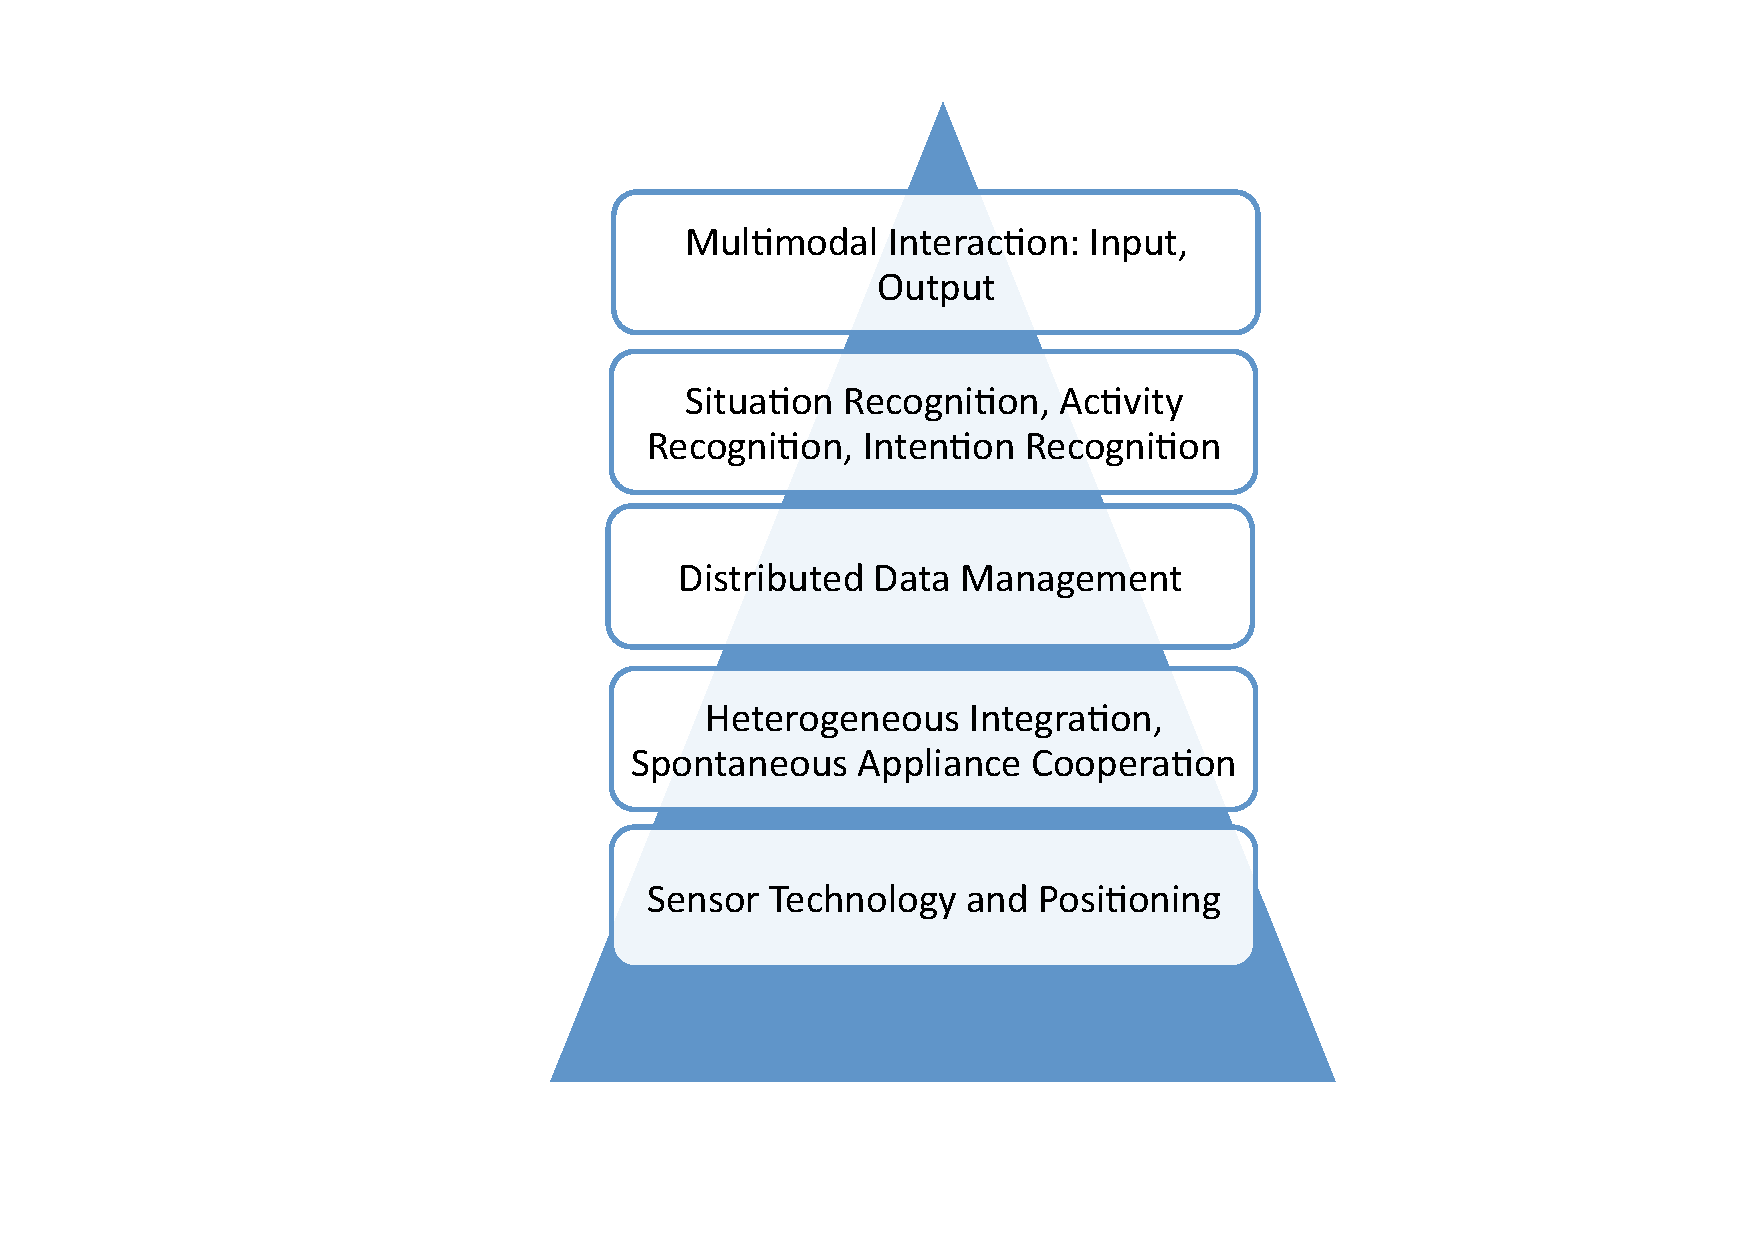
\includegraphics[width=0.65\textwidth]{figures/arch_aal.pdf}
    \caption{Architecture Overview of an Assistance System}
    \label{arch}
\end{figure}

The course uses many examples in pictures and videos to describe assistance systems and their properties and capabilities.
For explaining assistive technology to people without technical background, a layered architecture is used. The elementary architecture of an assistance system is described in Fig. \ref{arch}. The five layers are from the bottom up:
\begin{enumerate}
\item Sensor technology and positioning

There are many different and very small sensors which are integrated in many common devices, such as a positioning sensor in every smart phone.
\item Heterogeneous integration, spontaneous appliance cooperation

Devices have to be connected for sharing their data and information. Most device cooperations are predefined today. In the future devices will be probably cooperated spontaneously.
\item Distributed data management

For an intelligent environment, it is necessary to join and manage data. Otherwise, data should be evaluated at the device where the data are collected. This is especially important for the protection of data privacy.
\item Situation recognition, activity recognition, intention recognition

The recognition of situations, activities and user intentions is a difficult task for computers and works only in simple cases. This is currently a very active research area.
\item Multimodal interaction: input, output

The output possibilities are very diverse. For user input, the recognition of speech, gestures, and facial expression may be important in the future.
\end{enumerate}

For most of the participants in the AAL program, technical architectures like these are uncommon and not easy to understand. Therefore, everyday situations are used to illustrate the meaning behind the scheme. 

One example to explain the architecture is a parking assistant.
The positioning (lowermost layer in Fig. \ref{arch}) is realized by distance sensors integrated in the bumper.
Heterogeneous devices have to be interconnected (in the next layer): the sensors, the gear shift, the car radio and others.
The data of these devices have to be integrated (in the distributed data management layer). 
Recognizing the situation and the driver's intention: the driver puts in the reverse gear, so the driver possibly wants to park back-in.
The interaction with the user, i.e. driver (top layer in the architecture Fig. \ref{arch}) is done using the car radio. The output is commonly a beep with changing intervals.

Another example is used for explaining the current limits of modern robotics. The limits of robotics in aiding humans can be demonstrated by comparing a human world championship football match and a robotic world championship football match using video recordings.


\subsection{Special Issues}
The special problem of protecting privacy is widely discussed in the course. Privacy and the right of informational self-determination are important aspects in data management in Germany and is legally protected. In the context of assisted living, there is a correlation between assistance functionality and privacy. In simple terms, the more assistance functionality is provided, the more privacy is lost. Privacy awareness is an absolute necessity for AAL experts.

The importance of privacy in designing AAL products arose in a usability test at the RWTH Aachen University \cite{ZiWi14}, too.

\begin{figure}[ht]
    \centering
        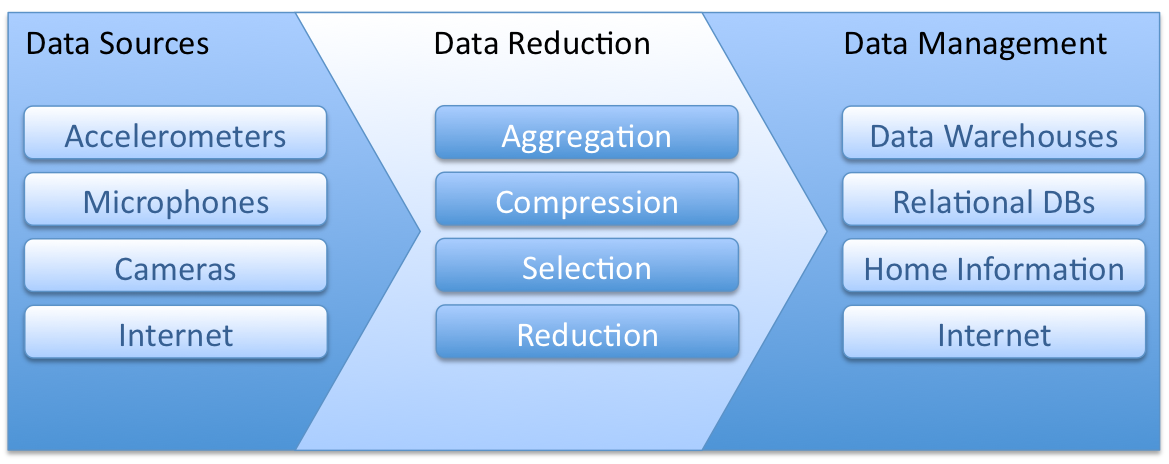
\includegraphics[width=1.0\textwidth]{figures/data-workflow.png}
    \caption{Data Workflow in Assistance Systems}
    \label{workflow}
\end{figure}

The possibilities designing AAL technology with decreased or minimized impact in losing privacy are explained using the data workflow in Fig. \ref{workflow}. On the left side, the data sources like sensors and cameras are depicted. On the right side, the handling, processing and analyzing as well as mining of interesting data using data warehouses, databases, and data mining tools are illustrated. Privacy-relevant data are collected at the sensors, cameras etc. and the loss of privacy happens during processing, analyzing and presentation of data at the latest. The collecting of data is possibly acceptable, if only the absolute relevant data is collected and data is immediately deleted after processing (also known as ``process and forget''). The data should be processed and forgotten as fast as possible. The best approach would be if the data never leave the sensor. Shrinking the amount of data leaving the private environment, there are operations current systems can handle, such as selection and aggregation of data (the middle column of Fig. \ref{workflow}).

\begin{figure}[ht]
    \centering
        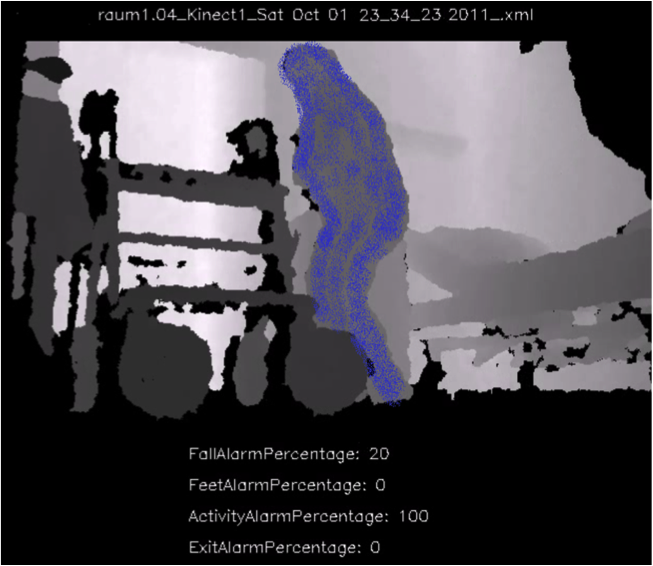
\includegraphics[width=0.7\textwidth]{figures/kinect.png}
    \caption{How private is this data? Fall detection using depth maps colored from white (far) to black (near) with the person subsequently blue-colored.}
    \label{kinect}
\end{figure}

The question, which data are possibly privacy-relevant, leads usually to a controversial discussion. In the course, an example of an AAL project concerning fall detection is used to illustrate relevant questions. The project, which was realized by the University of Rostock and partners \cite{MPBS12} uses a camera for fall detection. The participants are asked to discuss and evaluate the used technique. Fall detection is a good example to show problems in weighing up the advantages and disadvantages of an AAL solution. There are different solutions with different properties regarding limitations in user's mobility, privacy, user compliance, environment integration and reliability.

Participants usually discuss the following aspects:
\begin{itemize}
\item At which degree of fall endangering should the mobility of a person be observed or limited using an AAL solution? 
\item Is the fall detection suitable for a particular person? For instance, a wearable sensor may not be a good choice due to problems with compliance or unawares take off.
\item Does the AAL solution provide the needed level of privacy? Especially, camera-based systems produce undesirable images and videos (e.g. depth maps in Fig. \ref{kinect}). 
\end{itemize}

Fig. \ref{kinect} shows an image of a depth map of an elderly resident 

Exercising the exploration and evaluation of AAL technology, the participants should decide autonomous and independently: Is assisted living already reality or still vision from research. For this purpose, the participants have to develop an AAL solution for an own example mostly taken from their working environment.

\section{Scenarios and Participants' Reactions}\label{experiment}

Before the first seminar starts, participants are asked about their expectations on an AAL course.
Common answers are:
\begin{itemize}
\item Understanding the functionality of assistive technology and evaluating the benefits of such systems.
\item Knowing what AAL costs and how to finance AAL systems
\item Presentation, classification, and evaluation of systems regarding ethical aspects.
\item Declarations on general legal conditions
\item Information about available AAL solutions
\item Learning how to develop concepts for AAL projects regarding own interests within the course.
\item Exchanging experiences with other professions, learning more about other perspectives on AAL
\end{itemize}

After finishing the course, participants should be able to plan their own AAL concept. For deepening their understanding of technical principles, the participants were asked to develop AAL solutions in multi-professional groups. The participants have to develop the scenarios by describing the layers of the AAL reference architecture in Fig. \ref{arch}. The scenarios are the results of brainstorming in the groups. Later on, they were discussed in terms of technical practicability, desirability, as well as ethical and legal aspects and user compliance. The following three examples illustrate what kind of systems they have in mind.

\paragraph{First idea of an AAL scenario is called ``Communication against Isolation''\\}

It is about a home information base for elderly with special needs, e.g. limited mobility.

System properties and developing thoughts are:
\begin{itemize}
\item Information should be viewable on television or on tablet computer
\item using both devices as communication center and for video chats
\item using speech interface for home control
\item using always-on cameras and microphones in a Home Media Server environment
\item charging the tablet computer by a cradle or a mat for induction charging
\end{itemize}

\paragraph{Second scenario idea: ``Bedridden Person''\\}

Bedridden persons often have decubitus problems. An automatic system of sensors and actuating elements integrated in a mattress or mattress cover should help to avoid decubitus.

System properties and developing thoughts are:
\begin{itemize}
\item Recognizing decubitus using pressure sensors in a mattress cover is better than using sensors for blood flow in the clothes is better than camera-based recognition of decubitus
\item Actuating elements control the mattress achieving a pressure release
\item Further procedures: Informing or alerting a care service
\item Integration with vital signs using sensors in a bracelet or in clothes or in the mattress
\end{itemize}

\paragraph{Third scenario idea: ``Shower Assistant''\\}

Bathroom accidents and injuries are very common. A helping hand for washing and drying off someone is developed in this scenario.

System properties and developing thoughts are:
\begin{itemize}
\item Precondition: a seat in the shower
\item Sensor system: camera, microphone for speech control, infrared sensors in shower
\item Actuating elements: for controlling Water flow and temperature, automatic shower gel dispenser, handing towels,  automatic hair blower, handing new clothes
\item The shower assistant is not suitable for persons with a high care level. Otherwise, the system may be possible as a support for a nurse washing a patient, too.
\end{itemize}

The raised ethical aspects are further discussed in the next course ``Ethics and Law in AAL''.

After the courses, the participants were requested to answer questions about the courses, the lecturers, the organization, the material, and the personal conclusion.
Positive aspects were the engagement of the lecturers and organizers and the outcome for the participants. After the first trial of the courses, the study material was evaluated negatively. The explanations in the study material were too technically-oriented for most of the participants. These parts of the study material have been revised for the second course.

\section{Conclusions}
This paper describes experiences in designing, realizing and establishing a further education course for Ambient Assisted Living. The course was developed within the project BAAL funded by an initiative of the German Federal Ministry of Education and Research for developing and establishing education concepts for AAL. The paper is focused on how technical aspects of AAL can be taught for a target group without a technical background. Basis for the development of such a course is a profound analysis of educational demands, which include the target groups ability to understand technical principles and connect them to their professional knowledge in fields like health care system and housing industry.

Lessons learned: People without a technical background want to connect new knowledge in technical fields to their everyday life experience and their professional knowledge. The participant’s different perspectives on technical issues can be precious. That is why such participants have to be encouraged to think about technical solutions in complex AAL concepts and to enhance the multi-professional AAL discourse.

In the future, an interesting test could be the evaluation of assistive technology in a virtual reality environment. In \cite{SKMN11} an VR environment for AAL services for interacting and evaluating prototypes.

A look into the future of AAL job profiles has been done by \cite{PTK13}. These emerging job roles are described in detail and are related to existing professions. 
It will be interesting to see, if AAL experts becomes an accepted further education or if the AAL expert becomes a stand-alone profession.

\bibliographystyle{plain}
\bibliography{literature}


\end{document}
